\section{Una nueva regulación industrial}

%=============================================

A raíz de una nueva regulación industrial un fabricante debe rotular cada lote que produce según un valor numérico que lo caracteriza. Cada lote está conformado por “n” piezas. A cada una de ellas se le realiza una medición de volumen. La regulación considera que el lote es válido si más de la mitad de las piezas tienen el mismo volumen. En ese caso el rótulo deberá ser ese valor. De lo contrario el lote se descarta.

\subsection{Compilación y ejecución}
Para poder compilar el archivo part2.cpp ejecutar en consola de linux: g++ -o tp part2.cpp

Para poder ejecutarlo, en el directorio del ejecutable generado: ./tp PROCESO lotName

Donde PROCESO puede ser 'A', 'B' o 'C', sin comillas y lotName es el nombre del archivo del lote, que deberá estar en el mismo directorio.

\subsection{Proceso A}
Consiste en para cada pieza del lote contar cuántas de las restantes tienen el mismo volumen. Si alguna de las piezas corresponde al “elemento mayoritario”, se rotula el lote. De lo contrario se lo rechaza.
\subsubsection{Pseudocódigo}
\begin{verbatim}
    Llamar s a la cantidad de piezas del lote
    Inicializar un contador en q = 1, como cantidad de
    elementos con el mismo volumen
        Para cada pieza P_i del lote L:
            Para cada pieza P_j siguiente a P_i del lote L:
                Si el volumen v de las piezas P_i y P_j es el mismo:
                    incrementar q en 1.
            fin para
        Si q > s/2, finalizar la ejecución y etiquetar el lote con v.
        Si no, reiniciar q a 1 y avanzar en la iteración
        con la siguiente pieza.
        fin para
    Rechazar el lote.
\end{verbatim}


\subsubsection{Complejidad}
	Esta solución tiene una complejidad temporal de $\mathcal{O}(n^2)$, siendo $n$ la cantidad de piezas en el lote, pues hay dos ciclos anidados que se ejecutarían en función de esa variable. En el peor caso (no hay volumen mayoritario), para cada elemento $i$ del lote se hacen $(n-i)$ consultas. $n*(n-i) = n^2-i*n \Rightarrow \mathcal{O}(n^2)$. En el mejor caso, por otro lado, el ciclo se ejecutará una sola vez para un solo elemento, resultando  $\mathcal{O}(n)$.
Complejidad espacial: $\mathcal{O}(1)$ pues no se utilizan estructuras auxiliares.


%=====================================PROCESO B =========================================================
\subsection{Proceso B}
Consiste en ordenar las piezas por volumen y con ello luego reducir el tiempo de búsqueda del elemento mayoritario.
\subsubsection{Pseudocódigo}
\begin{verbatim}
    # pre: recibe un lote ordenado (lista de numeros), 
    Iniciar un contador q = 0
    Llamar k a la posición del elemento del medio del lote
    Mientras el elemento del lote P_i sea igual al elemento de k:
        incrementar q
        incrementar i
    fin mientras
    Mientras el elemento del lote P_i sea igual al elemento de k - 1:
        incrementar q
        decrementar i
    Si q es mayor que la mitad del tamaño del lote, 
       aprobar lote e indicar v = v[elemento de posición k]
    Sino, rechazar lote
\end{verbatim}
\subsubsection{Complejidad}
La complejidad temporal de este proceso depende del algoritmo de ordenamiento utilizado. El algoritmo en su peor caso es $\mathcal{O}(n)$. Si se utiliza mergesort o quicksort, que es $\mathcal{O}(n \log{}n): \mathcal{O}(n) + \mathcal{O}(n\log{}n) = \mathcal{O}(n \log{}n)$.
Complejidad espacial: $\mathcal{O}(1)$ pues no se utilizan estructuras auxiliares.

\subsection{Proceso C: División y Conquista}
Se utiliza una versión recursiva del algoritmo de votación del elemento mayoritario de Boyer-Moore para lograr una solución superadora a los procesos anteriormente propuestos,
teniendo que consultar únicamente dos veces cada pieza.\\\\
En el algoritmo original, cada elemento "tiene un voto". Se postula el primer elemento
como candidato a elemento mayoritario. Si el elemento "encuestado" es igual al candidato a elemento mayoritario, suma su voto. 
Si no, le resta un voto. Si la cantidad de votos llega a 0, el siguiente encuestado se postula como candidato y se continúa con la votación.
Al finalizar, se verifica que el candidato final sea efectivamente el elemento mayoritario contando la cantidad de apariciones. Si no lo es, no hay elemento mayoritario.\\
\\
Sea L una lista de elementos y M su elemento mayoritario (si existe). Si L está vacia, se devuelve el elemento de desempate D. Sino, se particiona L en pares y se incluye en una lista P sólo aquellos elementos que aparezcan dos veces en un mismo par (puesto que si la pareja no es idéntica, sus votos se cancelarían entre sí), 
entonces el elemento mayoritario en P es el mismo que en L. Como L puede no ser par, se utiliza en esos caso un elemento de desempate D igual al último elemento de L. 
Si L es par, D es nulo. Este D servirá para como un voto parcial para desempatar candidatos a M, dado el caso en alguno de los sub-problemas.

\subsubsection{Pseudocódigo}
\newcommand\bold[1]{\textbf{#1}}
\begin{Verbatim}[commandchars=\\\{\}]
ElementoMayoritario(lista, desempate=Ninguno):
    Si la lista está vacía:
        Retornar el elemento de desempate.
    Crear una lista vacía llamada pares.
    Si la lista tiene cantidad impar de elementos:
        Definir como elemento de desempate al último elemento de la lista.
    Para cada par de elementos en la lista:
       Si los dos elementos del par son idénticos:
          Añadir uno de los elementos a la lista pares
    Retornar ElementoMayoritario(pares, desempate)
    
ProcesoC():
    # Analiza la validez del lote e imprime la etiqueta del mismo si es
    # válido o "Rechazado" si no lo es
    R = ElementoMayoritario(lote)
    Si R es Ninguno, rechazar.    
    Contar la cantidad de apariciones de R en el lote.
    Si la cantidad de apariciones es mayor a la mitad del tamaño del lote:
       imprimir R en pantalla
   Sino, rechazar.
\end{Verbatim}

\subsubsection{Relación de recurrencia}
 En cada ejecución, se divide el problema en un subproblema $\Rightarrow q = a = 1$, y la cantidad de elementos en la lista es como máximo $n/2$ pues contiene uno o ningún número por cada par de elementos $\Rightarrow b=2$.\\
Formar los pares iterando sobre la lista de elementos es $\mathcal{O}(n)$, al igual que el contar después de la recursión 
la cantidad de apariciones de los candidatos $\Rightarrow f(n) = 2n = \mathcal{O}(n)$. 
	\begin{center}
	    $T(n) = T(n/2) + 2n $\\
	\end{center}
Aplicando el caso 3 del teorema maestro:
\begin{center}
    \doublespacing Si $f(n) = \Omega(n^{log_{b}{a}+e}),  e>0 \Rightarrow T(n) = \Theta(f(n))$\\
    \doublespacing$2n \stackrel{?}{=} \Omega(n^{0+e}),$ tomo $e=0.1$\\
    \doublespacing$2n = \Omega(n^{0.1})$ 
\end{center}
y para la condición de regularidad:
\begin{center}
    \doublespacing$\exists$ c $< 1$ para n grande / $a*f(n/b) \leq c*f(n) $\\
    \doublespacing$1 * 2n/2 \leq 2c*n$\\
    \doublespacing$n/(2c) \leq n$  $\forall$ c $\in (0,1)$\\
    \doublespacing$\therefore T = \mathcal{O}(n)$
\end{center}

\begin{figure}[!h]
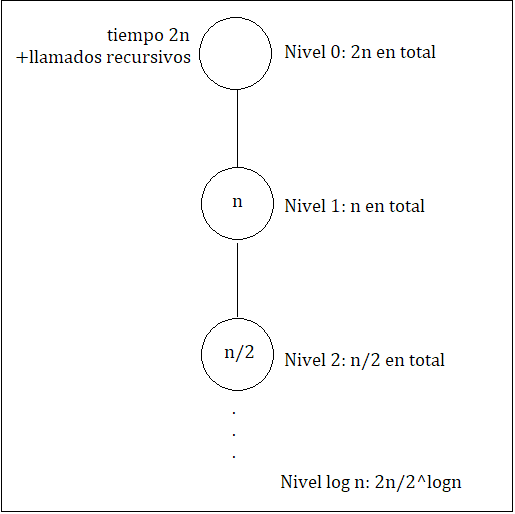
\includegraphics[width=7cm]{Informe/Imagenes/Parte2/proceso c.png}
\centering
\caption{Desenrollado de la recurrencia para el proceso C.}
\label{fig:desenrollado}
\end{figure}

Como se puede ver en la Figura \ref{fig:desenrollado}, con cada instancia de recursividad el trabajo a realizar en cada nivel va disminuyendo. En un nivel i, habrá una sola instancia de tamaño $2n/2^i$. Sumando los $\log{2}{n}$ niveles de la recursión, obtenemos la expresión:
\begin{center}

    \doublespacing$T(n) \leq \sum^{\log_{2}{n}-1}_{i=0} \frac{2*n}{2^i} = 4n$\\
    $\therefore T(n) = \mathcal{O}(n)$
\end{center}
\subsubsection{Complejidad}
Complejidad temporal: $\mathcal{O}(n)$ por lo desarrollado en la sección anterior.\\
Complejidad espacial: $\mathcal{O}(\log{n})$ por el uso de la pila de memoria. Se realizan como máximo $\log_{2}{n}$ llamados recursivos. 
